\documentclass[tikz]{standalone}
\usepackage{amsmath,amssymb,multirow}
\usetikzlibrary{shapes.misc, positioning,automata,arrows,calc,fit}
\tikzset{VertexStyle/.style = {draw,circle,thick,
		minimum size=1cm,
		font=\Large\bfseries},thick} 
\begin{document}
	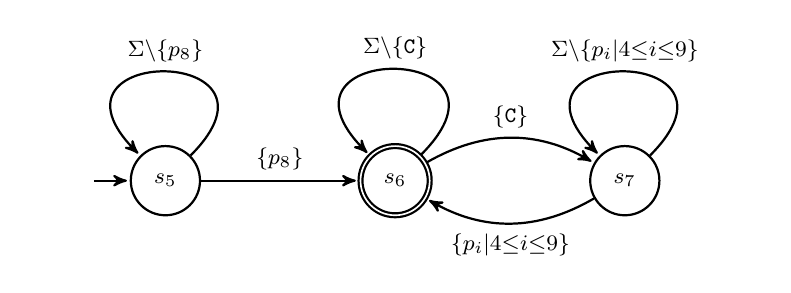
\begin{tikzpicture}[->,>=stealth',shorten >=1pt,thick,initial text=$ $,align=center,node distance=5mm,font=\footnotesize]
	\thickmuskip=0mu
	\node[state,initial] (SA) {$s_5$};
	\path (SA) edge[loop] node[midway,above] (W1) {$\Sigma\backslash\{p_8\}$} (SA);
	\node[state,accepting,right =2cm of SA] (ST) {$s_6$};
	\path (ST) edge[loop] node[midway,above] (W2) {$\Sigma\backslash\{\texttt{C}\}$} (ST);
	\draw[->] (SA) -- (ST) node[midway,above] {$ \{p_8\}$};
	\node[state,right=2cm of ST] (bot)  {$s_7$};
	\draw[->] (ST) edge [bend left] node[midway,above,sloped] {$\{\texttt{C}\}$}  (bot)  ; 
	\draw[->] (bot) 
	edge [bend left] node[midway,below,sloped] {$\{p_i|4\leq i\leq 9\}$} (ST)  ;
	\draw (bot) to [loop] node[above] (W3) {$\Sigma\backslash\{p_i|4\leq i\leq 9\}$} (bot);
	\end{tikzpicture}
\end{document}